\documentclass[11pt,a4paper]{article}

\usepackage[pdftex]{graphicx}
\usepackage{epstopdf}
\usepackage{subfigure}
\usepackage{amsmath,amsthm}
\usepackage{tikz}
\usetikzlibrary{babel}
\usetikzlibrary{shapes, arrows}
\textwidth= 15cm
\evensidemargin=0cm
\usepackage[spanish]{babel}
\usepackage[utf8]{inputenc}
\usepackage{textcomp}
\usepackage{amstext}
\usepackage{amsfonts}
\usepackage{amssymb}
\usepackage[hyperindex=true,breaklinks=true,colorlinks=true,linkcolor=blue]{hyperref}


\title{Linearization of state-space systems}
\author{Hector Garcia de Marina}
\date{Informal lecture notes, Sistemas Realimentados, Wednesday 7th 2020}


\tikzstyle{block} = [draw, rectangle, minimum width=6em]
\tikzstyle{sum} = [draw, fill=blue!20, circle, node distance=1cm]
\tikzstyle{input} = [coordinate]
\tikzstyle{output} = [coordinate]
\tikzstyle{pinstyle} = [pin edge={to-,thin,black}]

\newtheorem{definition}{Definition}
\newtheorem{theorem}{Theorem}
\newtheorem{algo}{Algorithm}


\begin{document}
\maketitle
\section{State-space systems}
We will focus on systems that can be described by quantifiable characteristics or states, e.g., temperature, velocity or voltage. These states might change over time. One might interact with a system via a quantifiable input, and one might measure some information from the states of the system via a quantifiable output.

Let us define $x(t)\in\mathbb{R}^n$, $y(t)\in\mathbb{R}^m$ and $u(t)\in\mathbb{R}^k$ as the stacked (signal) vector of states, the output, and the input of a system $\Sigma$ respectively. In particular, we will describe them as continuous signals over time, e.g., $x :[0,\infty) \to \mathbb{R}^n$. 

The system $\Sigma$ is a model that predicts the value of the states and the output over time. This prediction incorporates the impact of the input on the states and the output. We utilize differential equations as a tool to predict the evolution of the states of the system $\Sigma$ over time as follows
\begin{equation}
	\Sigma := \begin{cases}
		\dot x(t) =& f(x(t),u(t)) \\ y(t) =& g(x(t),u(t))
	\end{cases}, 
\label{eq: sigma}
\end{equation}
where $\dot x := \frac{\mathrm{d}}{\mathrm{dt}}(x(t))$ is the short notation for total derivative with respect to time, and $f: \mathbb{R}^n \times \mathbb{R}^k \to \mathbb{R}^n$ and $g: \mathbb{R}^n \times \mathbb{R}^k \to \mathbb{R}^m$ are functions.

We can represent the system $\Sigma$ as a block with input/output ports as in figure \ref{fig: sigma}.

\begin{figure}[!h]
\centering
\begin{tikzpicture}[auto, node distance=2cm,>=latex']
	\node [input, name=input] {};
	\node [block, right of=input] (system) {$\Sigma$};
	\node [output, right of=system] (output) {};
	\draw [draw,->] (input) -- node {$u(t)$} (system);
	\draw [->] (system) -- node [name=y] {$y(t)$}(output);
\end{tikzpicture}
	\caption{Input/output block diagram of system $\Sigma$.}
	\label{fig: sigma}
\end{figure}

\subsection{Exercise: Inverted pendulum}

We are going to derive $f$ and $g$ for the inverted pendulum.

First, we derive the equations of motion of the mass in the inverted pendulum system in figure \ref{fig: invpen} as a first step to figure out the system's functions $f$ and $g$. Consider that we can interact with the system with a torque $T$ applied on the base, the mass is under a friction force proportional to its speed, and we can only measure the angle $\theta$ from the system.

\begin{figure}[!h]
\centering
	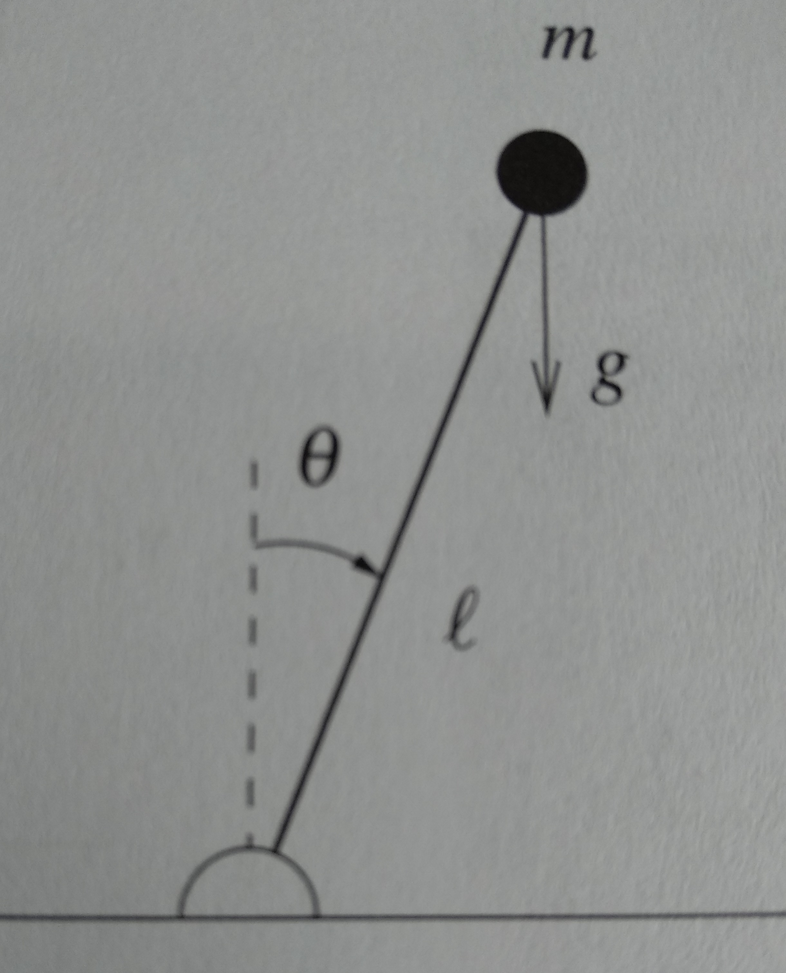
\includegraphics[scale=0.1]{./invpen.png}
	\caption{Inverted pendulum}
	\label{fig: invpen}
\end{figure}

We choose the angle $\theta$ with respect to the vertical to derive the dynamics of the inverted pendulum. Define $m, l, g,$ and $I\in\mathbb{R}$ as the mass, pendulum's lenght, gravity acceleration and inertia moment respectively. In particular, we have that $I = ml^2$, and we will exploit that $I \ddot\theta = \text{sum of torques}$. We have to consider three torques; namely: 1. Torque $T$ applied by us; 2. Torque $-b\dot\theta$ applied by the friction; 3. Torque $mgl \sin\theta$ applied by the gravitational forces, i.e., $mg$ is the force on the mass, times $\sin\theta$ since the force only applies perpendicular to the bar, and times $l$ to compute the resultant torque. Therefore the dynamics of the inverted pendulum are given by
\begin{equation}
\ddot\theta = \frac{1}{ml^2}\left(mgl\sin{\theta}-b\dot\theta + T\right).
	\label{eq: dyn}
\end{equation}

It looks reasonable to choose $\theta$ as one of our states to construct $x(t)$. In fact, since we have derived a second-order system, we will need $\dot\theta$ as a second state since we have the differential equation for its derivative $\ddot\theta$. Thus, let us define the state vector
\begin{equation}
x := \begin{bmatrix}\theta \\ \dot\theta \end{bmatrix},
\end{equation}
and since the torque $T$ is how we interact with the system, we choose the input $u(t) = T(t)$.

Now we are ready to construct the functions $f$ and $g$ in (\ref{eq: sigma}) for the inverted pendulum. In particular, we know that $f$ and $g$ only accepts as inputs/arguments the state space vector $x$ and the input $u$. On the left side of (\ref{eq: sigma}) we have the time derivative of $x(t)$, therefore
\begin{equation}
	\frac{\mathrm{d}}{\mathrm{dt}}\left(\begin{bmatrix}\theta \\ \dot\theta \end{bmatrix}\right) = f(x(t), u(t)) = \begin{bmatrix}f_1(x(t), u(t)) \\ f_2(x(t), u(t))\end{bmatrix}, \label{eq: fn}
\end{equation}
where $f_1 = \dot\theta$. Note that for the first row in (\ref{eq: fn}), on the left we have $\frac{\mathrm{d}}{\mathrm{dt}}\theta$, and on the right $f_1 = \dot\theta$ because $\dot\theta$ is actually a state, roughly speaking we can say that $\dot\theta(t) \in x(t)$. Unfortunatelly, we cannot say that $f_2 = \ddot\theta(t)$ because (roughly speaking) $\ddot\theta(t) \notin x(t)$. Nevertheless, we have that $f_2$ is given by the differential equation (\ref{eq: dyn}). Then, let me write explicitly $f$ as follows
\begin{equation}
	\frac{\mathrm{d}}{\mathrm{dt}}\left(\begin{bmatrix}\theta \\ \dot\theta \end{bmatrix}\right) =  f(x(t), u(t)) = \begin{bmatrix} \dot\theta \\ \frac{1}{ml^2}\left(mgl\sin{\theta}-b\dot\theta + T\right) \end{bmatrix}, \label{eq: f}
\end{equation}

The calculation of $g$ is more straightforward. We have established that we can only measure the angle, therefore $y(t) = \theta(t)$, i.e., 
\begin{equation}
g(x(t),u(t)) =  \theta(t).
	\label{eq: g}
\end{equation}

%A Python simulation of this dynamics can be found at \url{https://github.com/noether/aut_course}.

\section{Linearization of state-space systems}
Unfortunately, it is really (really) hard to calculate the analytic solution of $x(t)$ and $y(t)$ for a generic system $\Sigma$. Nevertheless, we will see that we can find the analytic solution for a state-space linear system.

The question then is whether we can relate a generic $\Sigma$ to a state-space linear system.

If $f(x,t)$ and $g(x,t)$ are real analytic around a specific point $(x^*,u^*)$, then we can approximate them around $(x^*,u^*)$ by a Taylor series expansion. This approximation is what we call \emph{linearization} if we stop at order one in the Taylor series
\begin{equation}
	\Sigma := \begin{cases}
	\dot x(t) =& f(x(t),u(t)) \\ y(t) =& g(x(t),u(t))
	\end{cases} \approx
	\begin{cases}
	\delta \dot x(t) &= A(t)\delta x(t) + B(t)\delta u(t) \\
	\delta y(t) &= C(t)\delta x(t) + D(t)\delta u(t)
	\end{cases} \quad x(t) \approx x^* + \delta x(t), u\approx u^* + \delta u(t), \nonumber
\end{equation}
where
\begin{align}
	A(t) &= \begin{bmatrix}
		\frac{\partial f_1}{\partial x_1} & \dots & \frac{\partial f_1}{\partial x_n} \\
		\vdots & \vdots & \vdots \\
		\frac{\partial f_n}{\partial x_1} & \dots & \frac{\partial f_n}{\partial x_n}
	\end{bmatrix}_{|_{x=x^*, u=u^*}} \nonumber \\
	B(t) &= \begin{bmatrix}
		\frac{\partial f_1}{\partial u_1} & \dots & \frac{\partial f_1}{\partial u_k} \\
		\vdots & \vdots & \vdots \\
		\frac{\partial f_k}{\partial u_1} & \dots & \frac{\partial f_k}{\partial u_k}
	\end{bmatrix}_{|_{x=x^*, u=u^*}} \nonumber \\
	C(t) &= \begin{bmatrix}
		\frac{\partial g_1}{\partial x_1} & \dots & \frac{\partial g_1}{\partial x_n} \\
		\vdots & \vdots & \vdots \\
		\frac{\partial g_m}{\partial x_1} & \dots & \frac{\partial g_m}{\partial x_n}
	\end{bmatrix}_{|_{x=x^*, u=u^*}} \nonumber \\
	D(t) &= \begin{bmatrix}
		\frac{\partial g_1}{\partial u_1} & \dots & \frac{\partial g_1}{\partial u_k} \\
		\vdots & \vdots & \vdots \\
		\frac{\partial g_m}{\partial u_1} & \dots & \frac{\partial g_m}{\partial u_k}
	\end{bmatrix}_{|_{x=x^*, u=u^*}} \nonumber
\end{align}
Roughly speaking, we calculate the sensitivity (up to first order) of $f$ and $g$ when we make a small variation on $x$ and $u$ around $(x^*,u^*)$. How close $(x,u)$ must be to $(x^*,u^*)$ depends on the particular system $\Sigma$. Later in the course, we will provide bounds for $\delta x$ and $\delta u$ such that we can apply with guarantees our control algorithms.

\subsection{Inverted pendulum, continuation}
We will see that, with the linearization, we can design controllers $u(t)$, i.e., a signal that our torque $T$ must follow, to drive the state of the pendulum where we wish. Let us define this point of interest as $x^* = \begin{bmatrix}\theta^* \\ 0\end{bmatrix}$, i.e., a fixed angle with (obviously) zero velocity. Indeed, this is an equilibrium point for the angle $\theta$. In order to have an equilibrium, we need to find a $u(t)$ in (\ref{eq: f}) such that $\frac{\mathrm{d}}{\mathrm{dt}}\left(\begin{bmatrix}\theta \\ \dot\theta \end{bmatrix}\right) = \begin{bmatrix}0 \\ 0 \end{bmatrix}$. A quick inspection to the dynamics (\ref{eq: dyn}) we have that
\begin{equation}
	u^* = T^* = -\frac{g}{l}\sin\theta^*,
\end{equation}
for example, for the vertical position of the pendulum corresponding to $\theta^* = 0$ we have that $T^*=0$, i.e., $x^* = \begin{bmatrix}0\\0\end{bmatrix}$ and $u^* = 0$.

The calculation of the matrices $A,B,C,$ and $D$ are the corresponding Jacobians for $(\ref{eq: f})$ and $(\ref{eq: g})$, i.e.,

\begin{align}
\frac{\partial f_1}{\partial x_1} &= 0 \nonumber \\
\frac{\partial f_1}{\partial x_2} &= 1 \nonumber \\
\frac{\partial f_2}{\partial x_1} &= \frac{g}{l}\cos\theta \nonumber \\
\frac{\partial f_2}{\partial x_2} &= -\frac{b}{ml^2} \nonumber \\
\frac{\partial f_1}{\partial u_1} &= 0 \nonumber \\
\frac{\partial f_2}{\partial u_1} &= 1 \nonumber \\
\frac{\partial g_1}{\partial x_1} &= 1 \nonumber \\
\frac{\partial g_1}{\partial x_2} &= 0 \nonumber \\
\frac{\partial g_1}{\partial u_1} &= 0, \nonumber
\end{align}
therefore we can arrive at
\begin{align}
	\frac{\mathrm{d}}{\mathrm{dt}}\left(\begin{bmatrix}\delta\theta \\ \dot\delta\theta \end{bmatrix}\right) &= \begin{bmatrix}0 & 1 \\ \frac{g}{l}\cos\theta & -\frac{b}{ml^2} \end{bmatrix}_{|_{\theta=\theta^*}} \begin{bmatrix}\delta\theta \\ \dot\delta\theta \end{bmatrix} + \begin{bmatrix}0 \\ 1 \end{bmatrix} \delta T \nonumber \\
		\delta y &= \begin{bmatrix}1 & 0\end{bmatrix}\begin{bmatrix}\delta\theta \\ \dot\delta\theta \end{bmatrix} + 0 \, \delta T,
\end{align}
to model the dynamics of $x(t)$ and the output $y(t)$ around the points $x^*$ and $u^*$.

Finally, we would like to hightlight that the Jacobians can have time-varying elements, and still have a linear system. For example, we can consider that the lenght $l$ depends on the time explicitly, e.g., $l(t) = l + \sin(t)$. In such a case, we would have a $A(t)$.

\end{document}
